\section{Data}
The dataset is provided with the \emph{Turtle Recall: Conservation Challenge}\footnote{\url{https://zindi.africa/competitions/turtle-recall-conservation-challenge/data}} and consists of images of turtle faces. The images are labelled, each turtle has a unique ID. Besides the angle from which the image was shot (top, right, left) and the ID, no further info is provided about the images.

The images themselves have three colour channels, come in different sizes, and many have timestamps or handwritten identification tags in the background. They are split in three parts: a set of images for training, one for testing, and a large set of extra images.

The training set consists of 2145 images from 100 unique turtles. The set with the extra images comes with an additional almost 11000 images from 2231 different turtles, some already contained in the train set. This yields a total of about 13000 images and 2265 turtles. The test set only comes with images but without the annotation of turtle IDs, as it is meant to be used for model evaluation in the priced competition. However, this means that the test images are without use for our purpose.

Because the training set is rather small, we also make use of the extra images. A quick exploratory analysis shows that the dataset is both hugely unbalanced and that there are only less than 6 images per turtle on average, with a median number of 3 images per turtle. Because such a small amount of data per class will likely lead to very poor approximation results, we decide not to use the entire available data.


\subsection{Preprocessing}
Before actually using the images and feeding them into a neural net, we need to perform some necessary as well as some optional preprocessing steps in order to bring the image data into a more helpful format.

As a first step, we get rid of any turtles with less than a specified number of images in the dataset. We require each turtle to be represented by at least 10 images in the dataset. This reduces the total number of turtles to 253 and the total number of images to roughly 5000. Turtles now have an average of 20 images and a median of 14 images. There is still a considerable imbalance in the data, as can be seen in figure \ref{fig:images_per_turtle}.

\begin{figure}[h]
    \centering
    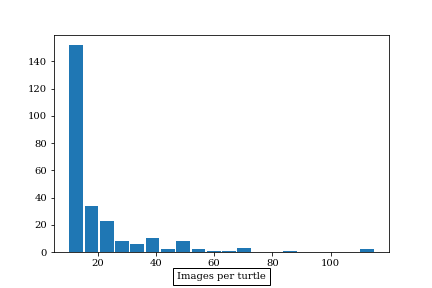
\includegraphics[width=12cm]{images/images_per_turtle.png}
    \caption[Number of images per turtle]{Number of images per turtle. The left skew of the distribution means there are many images with the minimum amount of images, while only a few have considerably more.}
    \label{fig:images_per_turtle}
\end{figure}

We further crop and resize the images such that they are all in the same shape and size, namely $224\times224$ pixels. Before doing any computations on the image data, we also convert them to numerical arrays, yielding us a three-dimensional array of size $224\times224\times3$ for each used image. Since the colours are in the RGB colour space, the values are now in the range \numrange{0}{255}, which we normalise to a range of \numrange{0}{1}. This has been shown to increase training speed of deep networks \citep{Ioffe2015}. We further apply a one-hot encoding to the classes, as the alpha-numerical strings the turtle IDs are supplied in are rather meaningless to a neural net. At this point, we are technically ready to feed the images into a network for training.


\subsection{Data Augmentation}
The dataset, unfortunately, contains very little data unevenly distributed among the classes. A low number of training examples per class can lead to the class not being learned efficiently and may even impede the entire training process \citep{Huh2016}. To avoid this, we apply a set of basic augmentation techniques to multiply the data available for training:

\begin{description}
    \item[Image rotation] We rotate the images by 90, 180, and 270 degrees. This immediately quadruples the available data. The basic characteristics of the pattern on the head of the turtle are preserved.
    \item[Gaussian filter] We also apply a Gaussian filter to introduce a blur and reduce detail in the image. Mathematically, this is the same as convolving the images with a Gaussian function.
    \item[Random HSV] The HSV colour space uses hue, saturation, and value to describe colours, whereas the RGB colour model uses a linear combination of the colours red, green, and blue to describe the same. We transform the RGB values to HSV, randomly modify them within a specified range, and convert back to RGB.
    \item[Additive noise] Lastly, we add random numerical values, sampled from a normal distribution with very low standard deviation, to the existing image values, followed by clipping the values within range \numrange{0}{1} (our normalisation range).
\end{description}

Applying the above techniques, we have enhanced our dataset and also somewhat shifted the distribution of images per turtle to be more desirable. Further common augmentation techniques include random brightness shifts, grey level mapping, histogram equalisation, image shifting and shearing. Example images of the used augmentations can be seen in appendix \ref{apx:augmentedImages}.